% CHAPTER 1
\chapter{VALIDATION IN TEST CASE}
\label{chp:4}
\section{P.M.Anderson 9 Bus Test Case}
\subsection{System Properties}
In order to understand frequency dynamics better, P.M. Anderson test case has been used in the study. The single line diagram of the system is given in Figure \ref{ieee_9_bus}. The test case consists of three generators and three loads. Generators in the system are connected to 230 kV high voltage network with transformers.\par
\begin{figure}[h!]
	\centering
	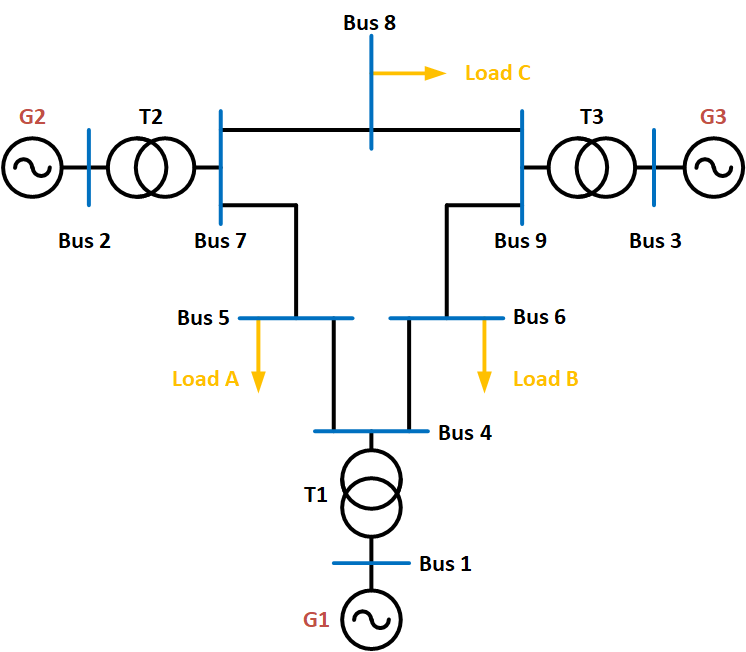
\includegraphics[width=.85\linewidth]{ieee_9_bus.png}
	\caption{P.M.Anderson Test Case}
	\label{ieee_9_bus}
\end{figure}
The biggest generator in the system is a hydropower plant with a power rating of 247.5 MVA. The remaining ones are steam generators. The power ratings of the generators are given in Table \ref{generatorproperties}.\par
\begin{table}[h!]
	\centering
	\begin{tabular}{ccc}
		\hline
		\textbf{Generators} & \textbf{Power Rating (MVA)} & \textbf{Plant Type} \\ \hline
		Gen 1               & 247.5                       & Hydro				\\
		Gen 2               & 192                         & Steam               \\
		Gen 3               & 128                         & Steam               \\ \hline
	\end{tabular}
	\caption{Generator Properties of Test System}
	\label{generatorproperties}
\end{table}
The loads in the system are connected directly to the high voltage network. The active and reactive power ratings of the loads are listed in Table \ref{loadproperties}.
\begin{table}[h!]
	\centering
	\begin{tabular}{ccc}
		\hline
		\textbf{Generators} & \textbf{Active Power (MW)}  & \textbf{Reactive Power (MVAr)} \\ \hline
		Load A              & 125                      	  & 50				 \\
		Load B              & 90                          & 30                \\
		Load C              & 100                         & 35                \\ \hline
	\end{tabular}
	\caption{Load Properties of Test System}
	\label{loadproperties}
\end{table}
\subsection{Load Flow Analysis for Base Case}
Successful grid operation requires a load flow analysis in order to ensure that bus voltages are inside the allowed band and power flows are below the power carrying capabilities of the lines. Load flow results are given in Table \ref{loadflow_case1}.
\begin{table}[h!]
	\centering
	\begin{tabular}{cclccccc}
		\hline
		Bus \# & Bus Type & \multicolumn{1}{c}{Voltage} & Angle & Pg    & Qg     & Pl  & Ql \\ \hline
		1      & SL       & \multicolumn{1}{c}{1.04}    & 0     & 71.65 & 27.05  & 0   & 0  \\
		2      & PV       & \multicolumn{1}{c}{1.025}   & 9.28  & 163   & 6.65   & 0   & 0  \\
		3      & PV       & \multicolumn{1}{c}{1.025}   & 4.66  & 85    & -10.86 & 0   & 0  \\
		4      & PQ       & 1.0258                      & -2.22 & 0     & 0      & 0   & 0  \\
		5      & PQ       & 0.9956                      & -3.99 & 0     & 0      & 125 & 50 \\
		6      & PQ       & 1.0126                      & -3.69 & 0     & 0      & 90  & 30 \\
		7      & PQ       & 1.0258                      & 3.72  & 0     & 0      & 0   & 0  \\
		8      & PQ       & 1.0159                      & 0.73  & 0     & 0      & 100 & 35 \\
		9      & PQ       & 1.0323                      & 1.97  & 0     & 0      & 0   & 0  \\ \hline
	\end{tabular}
	\caption{Load Flow Results in Base Case}
	\label{loadflow_case1}
\end{table}
\subsection{Load Connection}
It is obvious that power system networks experience high RoCoF when either high amount of generation trips or high amount of load connects to system. These two main event can be used in the simulation to create frequency disturbances. Since the simulation in Simulink environment slows down with the increasing amount of generators, the disturbances are created with load connections.\par
\begin{table}[]
	\centering
	\begin{tabular}{ll}
		\hline
		Total System Load                      & 315 MW    \\
		Generator Droop Settings               & 5\%       \\
		Stored Kinetic Energy at Nominal Speed & 3.305 GWs \\
		Gen 1 Inertia Constant                 & 9.5515 s  \\
		Gen 2 Inertia Constant                 & 3.9216 s  \\
		Gen 3 Inertia Constant                 & 2.7665 s  \\ \hline
	\end{tabular}
	\caption{System Dynamical Properties}
	\label{systemdynamicaldata}
\end{table}
System dynamical properties are listed in Table \ref{systemdynamicaldata}. Power generation references are determined based on the load flow of powergui toolbox. Machine initialization toolbox is also used to initiate the state of generators in the system. However, the system does not start with the steady state. Still, system goes to steady state within a few seconds. Frequency of the network is disturbed with a load connection in the t=10 seconds in order to observe the frequency stability of the system. For 10\% load connection, a load of 31.5 MW is connected to system from Bus 6. Location of the additional load is depicted in Figure \ref{ieee_9_bus_load}.\par
\begin{figure}[h!]
	\centering
	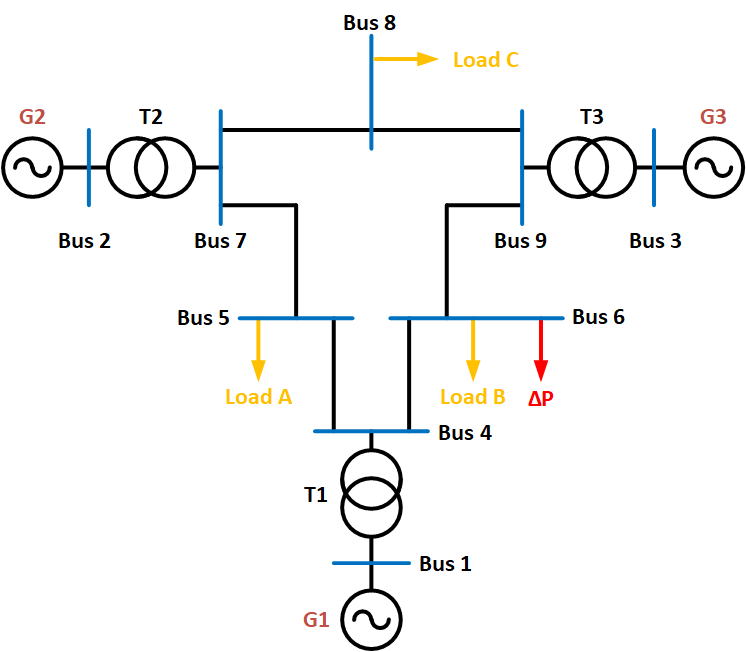
\includegraphics[width=.85\linewidth]{ieee_9_bus_load_position.png}
	\caption{Location of the Additional Load}
	\label{ieee_9_bus_load}
\end{figure}
According to the 10\% load connection to system, generator frequencies are shown in Figure \ref{genfreqcase1}. Frequency of generator 1 is the most smooth one due to its huge inertia constant. Meanwhile, the generator 2 and generator 3 follow the frequency of generator 1 even though they oscillate with each other. \par
\begin{figure}[h!]
	\centering
	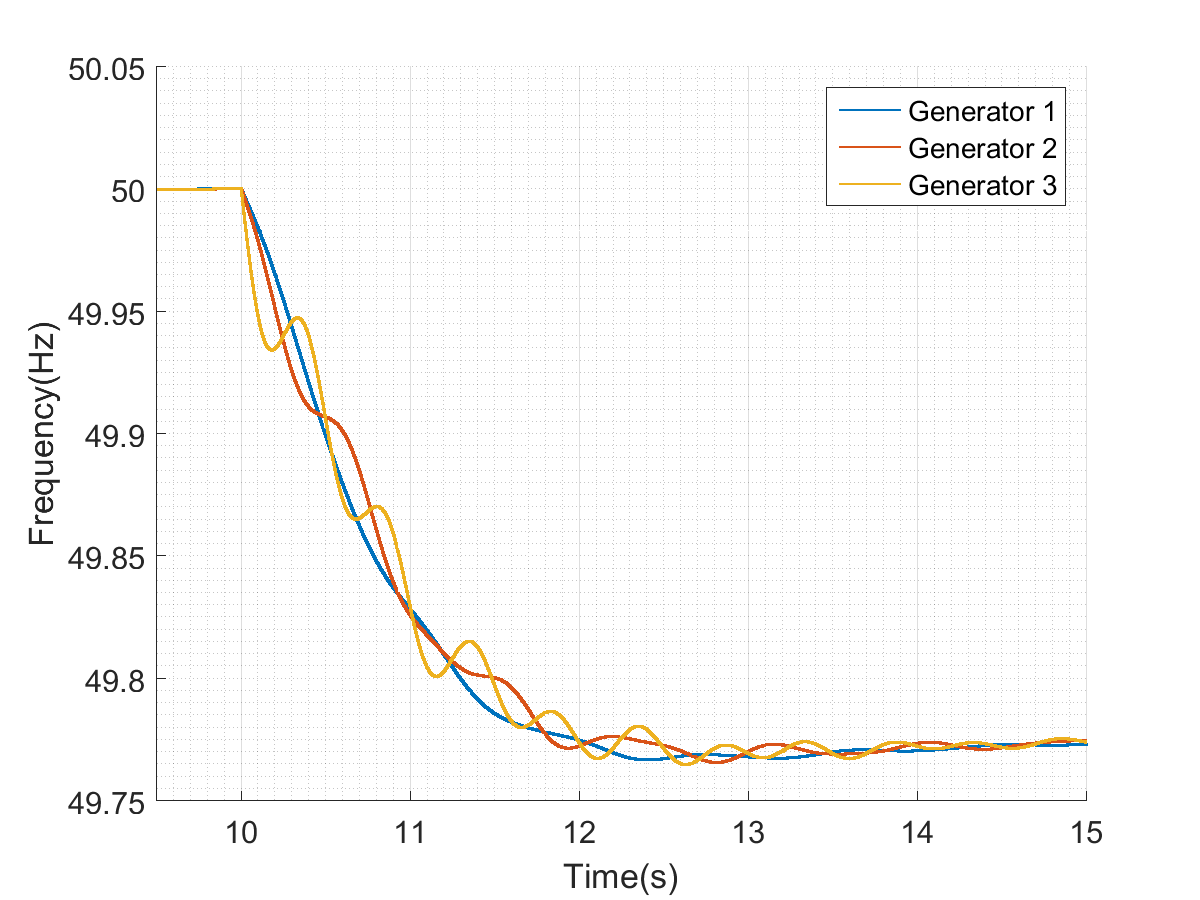
\includegraphics[width=.85\linewidth]{Case1_Generator_Freq.png}
	\caption{Generator Frequencies for 10\% Load Connection}
	\label{genfreqcase1}
\end{figure}
In the system, frequency of Bus 1 can be assumed as constant throughout the network since the system is small enough to assume a single frequency. This assumption can be verified by comparing the frequencies in Buses 1, 5 and 6. Figure \ref{genfreqcase1_loadgen} shows the frequency of the generator 1 frequency as well as the load frequencies captured with Simulink PLL block. The only difference is the instant following the load connection. The sharp frequency decline delays the PLL loop to capture the frequnecy. 
\begin{figure}[h!]
	\centering
	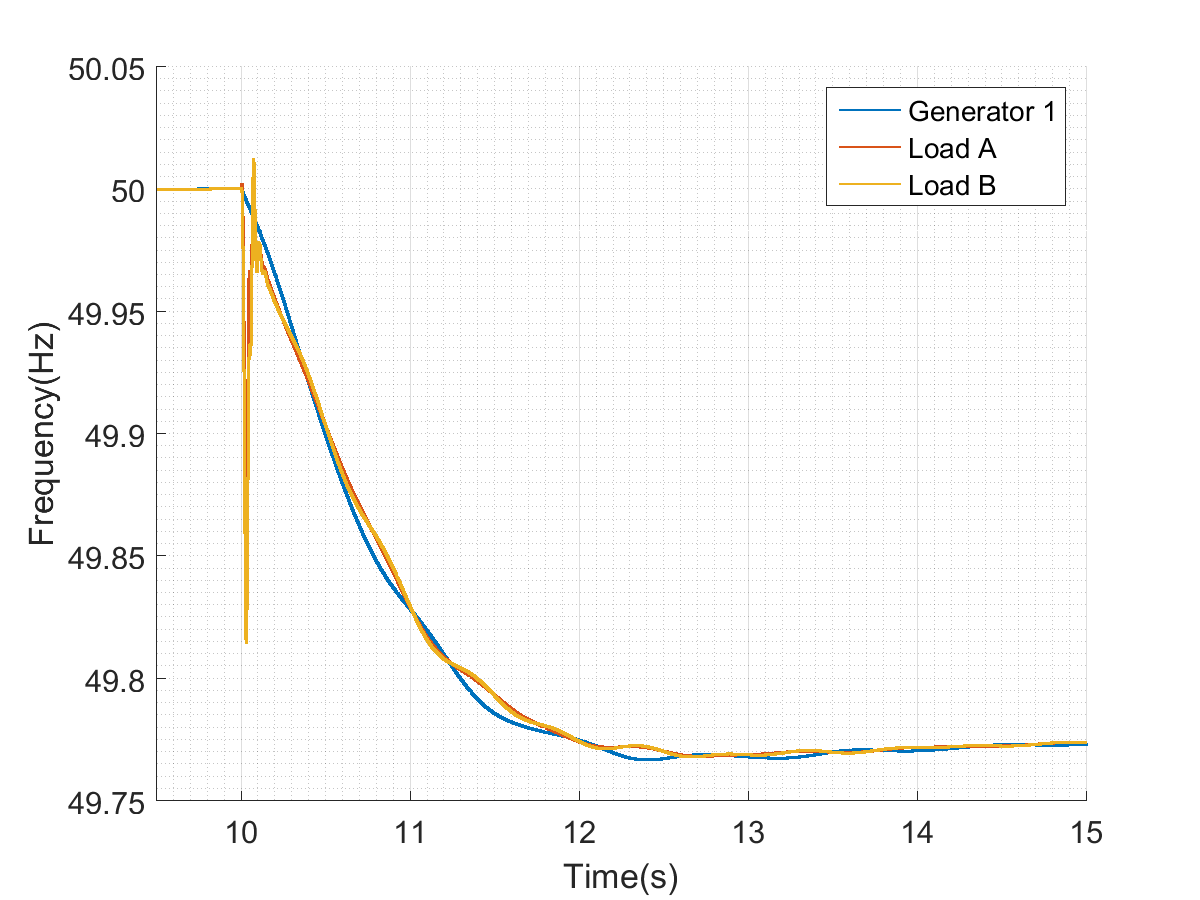
\includegraphics[width=.85\linewidth]{Case1_Load_Gen_Freq.png}
	\caption{Frequencies in Generator 1, Load A and Load B}
	\label{genfreqcase1_loadgen}
\end{figure}
\section{Modified Case}
In this case, the P.M. Anderson test case is modified such that a wind farm consists of 20 wind turbine is connected to network. Wind farm is connected to Bus 5. Modified system is depicted in the Figure \ref{ieee_9_bus_case2}. In this case, generator 2 and 3 are still assigned to same power values meanwhile generator 1 decreases its generation. 
\begin{figure}[h!]
	\centering
	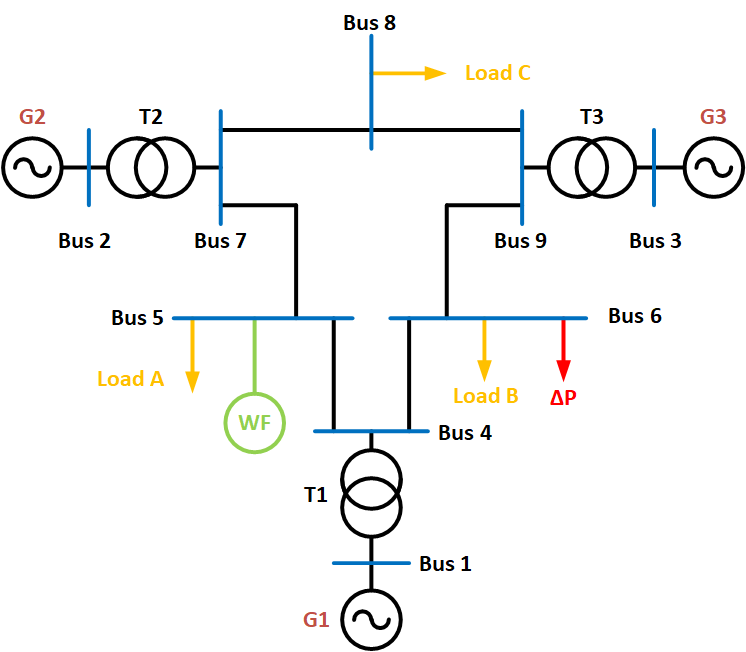
\includegraphics[width=.85\linewidth]{ieee_9_bus_modified.png}
	\caption{Modified System Single Line Diagram}
	\label{ieee_9_bus_case2}
\end{figure}
\subsection{Load Flow Analysis for Modified Case}
\begin{table}[h!]
	\centering
	\begin{tabular}{cclccccc}
		\hline
		Bus \# & Bus Type & \multicolumn{1}{c}{Voltage} & Angle & Pg    & Qg     & Pl  & Ql \\ \hline
		1      & SL       & \multicolumn{1}{c}{1.04}    & 0     & 38.06 & 25.07  & 0   & 0  \\
		2      & PV       & \multicolumn{1}{c}{1.025}   & 11.33 & 163   & 6.65   & 0   & 0  \\
		3      & PV       & \multicolumn{1}{c}{1.025}   & 6.32  & 85    & -10.86 & 0   & 0  \\
		4      & PQ       & 1.0263                      & -1.18 & 0     & 0      & 0   & 0  \\
		5      & PQ       & 0.9995                      & -1.54 & 0     & 0      & 125 & 50 \\
		6      & PQ       & 1.0128                      & -2.43 & 0     & 0      & 90  & 30 \\
		7      & PQ       & 1.0266                      & 5.77  & 0     & 0      & 0   & 0  \\
		8      & PQ       & 1.0164                      & 2.62  & 0     & 0      & 100 & 35 \\
		9      & PQ       & 1.0326                      & 3.62  & 0     & 0      & 0   & 0  \\ \hline
	\end{tabular}
	\caption{Load Flow Results for Modified Case}
	\label{loadflow_case2}
\end{table}